When working with time series, we often want to determine whether one series causes changes in another. To find this relationship, measuring a cross-correlation and finding a lag is one way how to do it. Lag represents when change in one data series transfers to the other several periods later. 

To ensure a cross-correlation calculation makes sense, first I have to determine, whether are the data stationary. A stationary time series is one whose properties do not depend on the time at which the series is observed\cite{hyndman5forecast}. More precisely, if y\textsubscript{t} is a stationary time series, then for all \textit{s}, the distribution of \textit{(y\textsubscript{t},…,y\textsubscript{t+s})} does not depend on \textit{t}.

To determine whether my data are stationary, I've used the Dickey-Fuller test method of tseries package in R. Results can be seen in the table \ref{table:stationarity_table} 

\begin{table}
\centering
\begin{tabular}{ |p{3cm}||p{3cm}|p{3cm}|  }
 \hline
 \multicolumn{3}{|c|}{Stationarity test of web frameworks sentiment data} \\
 \hline
 Framework & Dickey-Fuller & p-value\\
 \hline
 NodeJS   & -2.6775    &0.2964\\ \hline
 AngularJS &   -3.883  & 0.0199\\ \hline
 EmberJS & -4.0783 & 0.0199\\ \hline
 VueJS    &-3.438 & 0.0646\\ \hline
 CakePHP&   -3.480  & 0.04847\\ \hline
 Laravel& -2.57  & 0.3431\\ \hline
 Symfony& -4.3979  & 0.01\\ \hline
\end{tabular}
\caption{Stationarity test of sentiment}
\label{table:stationarity_table}
\end{table}

As we can see, some data are not stationary, therefore I can't calculate the cross-correlation on them in this state. To transform non-stationary data into stationary, 2 approaches can be used. These are differencing and transforming. For example sentiment change for NodeJS has a p-value higher than 0.05 what indicates non-stationarity. I've taken these data and differenced the values. I've executed both, seasonal differencing and stationary differencing although seasonal probably was not needed because the data should not be dependant on the season. New differenced values do appear to be stationary in mean and variance, as the level and the variance of the series stays roughly constant over time. Sentiment for NodeJS before and after differencing can be seen in Figure \ref{fig:NodeJS_Sentiment_before_after}

\begin{figure}%
    \centering
    \subfloat[Before differencing]{{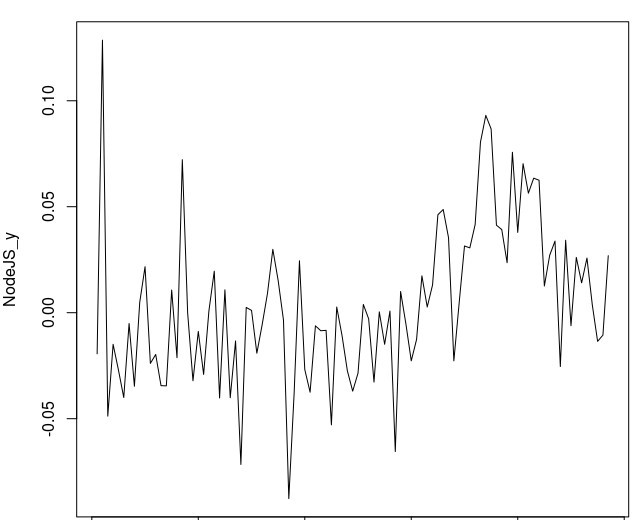
\includegraphics[width=6cm]{NodeJS_beforeDiff.jpg} }}%
    \qquad
    \subfloat[After differencing]{{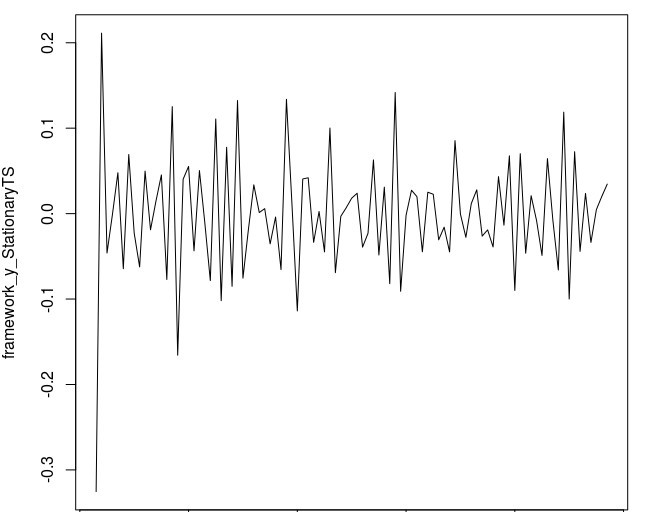
\includegraphics[width=6cm]{NodeJS_afterDiff.jpg} }}%
    \caption{NodeJS monthly sentiment values}%
    \label{fig:NodeJS_Sentiment_before_after}%
\end{figure}

Same procedure needed to be done with the "number of releases per month" data and afterwards, cross-correlation could be executed. For this task I've used ccf method in R. 